% Fixed-population analysis. Numerical inputs: generated/ch3_transport_report.json.
\chapter{Horizontal transport and displacement scaling}
\label{ch:fixed-transport}
% Generated by scripts/tesi/ch03_fixed_transport/write_ch3_text.py
% Chapter prose is hand-written; only these values are generated.
\newcommand{\ChThreeClosedAltShiftMax}{0.051}
\newcommand{\ChThreeClosedAltShiftMin}{0.021}
\newcommand{\ChThreeCohortBiasMaxPct}{2.0}
\newcommand{\ChThreeCohortBiasMinPct}{1.8}
\newcommand{\ChThreeCohortShiftMax}{0.0177}
\newcommand{\ChThreeCohortShiftMin}{0.0164}
\newcommand{\ChThreeEligibleClosed}{87,807}
\newcommand{\ChThreeEligibleClosedPct}{56.6}
\newcommand{\ChThreeEligibleOpen}{67,003}
\newcommand{\ChThreeEligibleOpenPct}{43.2}
\newcommand{\ChThreeEligibleUnknown}{275}
\newcommand{\ChThreeGeneralFitLagMax}{30000}
\newcommand{\ChThreeGeneralFitLagMin}{10}
\newcommand{\ChThreeGeneralLastFitLag}{28440}
\newcommand{\ChThreeHangClosedFracMain}{76.5}
\newcommand{\ChThreeHangClosedFracStart}{64.0}
\newcommand{\ChThreeHangCohortOverlapPct}{99.7}
\newcommand{\ChThreeHangGeneralGroups}{7}
\newcommand{\ChThreeHangGeneralHurst}{0.841 [0.816, 0.855]}
\newcommand{\ChThreeHangGeneralReplicates}{998}
\newcommand{\ChThreeHangGeneralRms}{0.075}
\newcommand{\ChThreeHangGeneralRmsRatio}{1.19}
\newcommand{\ChThreeHangKurtEEnd}{4.03}
\newcommand{\ChThreeHangKurtEStart}{-0.60}
\newcommand{\ChThreeHangKurtNEnd}{2.24}
\newcommand{\ChThreeHangKurtNStart}{-0.72}
\newcommand{\ChThreeHangLastSupportLag}{43200}
\newcommand{\ChThreeHangLocalMinH}{0.57}
\newcommand{\ChThreeHangLocalMinLag}{320}
\newcommand{\ChThreeHangMomentContrast}{-0.0085 [-0.0112, -0.0057]}
\newcommand{\ChThreeHangMomentRmsMax}{0.126}
\newcommand{\ChThreeHangMomentRmsMin}{0.011}
\newcommand{\ChThreeHangPriorInterp}{9,648}
\newcommand{\ChThreeHangQuantRatioEnd}{0.233}
\newcommand{\ChThreeHangQuantRatioMax}{0.385}
\newcommand{\ChThreeHangQuantRatioMaxLag}{1970}
\newcommand{\ChThreeHangQuantRatioMin}{0.192}
\newcommand{\ChThreeHangQuantRatioMinLag}{90}
\newcommand{\ChThreeHangQuantRatioStart}{0.472}
\newcommand{\ChThreeHangQuantRmsMax}{0.101}
\newcommand{\ChThreeHangQuantRmsMin}{0.037}
\newcommand{\ChThreeMainClosed}{28,234}
\newcommand{\ChThreeMainClosedPct}{61.0}
\newcommand{\ChThreeMainOpen}{17,961}
\newcommand{\ChThreeMainOpenPct}{38.8}
\newcommand{\ChThreeMainUnknown}{78}
\newcommand{\ChThreeOpenAltShiftMax}{0.064}
\newcommand{\ChThreeOpenAltShiftMin}{0.051}
\newcommand{\ChThreeParaClosedFracMain}{61.0}
\newcommand{\ChThreeParaClosedFracStart}{56.6}
\newcommand{\ChThreeParaCohortOverlapPct}{99.6}
\newcommand{\ChThreeParaGeneralHurst}{0.869 [0.864, 0.874]}
\newcommand{\ChThreeParaGeneralRms}{0.038}
\newcommand{\ChThreeParaGeneralRmsRatio}{1.09}
\newcommand{\ChThreeParaKurtEEnd}{2.77}
\newcommand{\ChThreeParaKurtEStart}{-0.68}
\newcommand{\ChThreeParaKurtNEnd}{0.94}
\newcommand{\ChThreeParaKurtNStart}{-0.97}
\newcommand{\ChThreeParaLastSupportLag}{32690}
\newcommand{\ChThreeParaLocalMinH}{0.66}
\newcommand{\ChThreeParaLocalMinLag}{110}
\newcommand{\ChThreeParaMomentContrast}{0.0095 [0.0086, 0.0105]}
\newcommand{\ChThreeParaMomentRmsMax}{0.079}
\newcommand{\ChThreeParaMomentRmsMin}{0.010}
\newcommand{\ChThreeParaPriorInterp}{355,170}
\newcommand{\ChThreeParaQuantRatioEnd}{0.205}
\newcommand{\ChThreeParaQuantRatioMax}{0.398}
\newcommand{\ChThreeParaQuantRatioMaxLag}{1970}
\newcommand{\ChThreeParaQuantRatioMin}{0.244}
\newcommand{\ChThreeParaQuantRatioMinLag}{100}
\newcommand{\ChThreeParaQuantRatioStart}{0.510}
\newcommand{\ChThreeParaQuantRmsMax}{0.084}
\newcommand{\ChThreeParaQuantRmsMin}{0.023}
\newcommand{\ChThreeTaskContrastMax}{0.129}
\newcommand{\ChThreeTaskContrastMin}{0.023}
\newcommand{\ChThreeTaskGapHigh}{0.023 [0.021, 0.024]}
\newcommand{\ChThreeTaskGapHills}{0.129 [0.125, 0.132]}
\newcommand{\ChThreeTaskGapLow}{0.048 [0.046, 0.049]}
\newcommand{\ChThreeTaskGapPlains}{0.128 [0.120, 0.138]}


Horizontal transport depends on both the distance covered and its growth with time.
We measure the mean-square displacement (MSD), its dependence on circuit type and
initial altitude, and the scaling of the displacement distribution. Paragliders and
hang gliders are analysed separately.

\section{Mean-square displacement}
\label{sec:fixed-msd}
\subsection{Estimator and temporal resolution}

Let $\boldsymbol{x}_f(t)=(E_f(t),N_f(t))$ be the cleaned horizontal trajectory of flight
$f$. Within its retained continuous segments, define
$\Delta\boldsymbol{x}_{fi}(\tau)=\boldsymbol{x}_f(t_i+\tau)-\boldsymbol{x}_f(t_i)$
and $R_{fi}(\tau)=|\Delta\boldsymbol{x}_{fi}(\tau)|$. For the contributing flights
$\mathcal C(\tau)$, let $N(\tau)=|\mathcal C(\tau)|$ and $n_f(\tau)$ be the number
of valid increments. The time-averaged MSD of a flight and its population mean are
\begin{equation}
 m_f(\tau)=\frac{1}{n_f(\tau)}\sum_{i=1}^{n_f(\tau)}R_{fi}(\tau)^2,
 \qquad M_2(\tau)=\frac{1}{N(\tau)}\sum_{f\in\mathcal C(\tau)}m_f(\tau).
 \label{eq:fixed-msd}
\end{equation}
This \emph{equal-flight} average gives each flight total weight $1/N(\tau)$, so long
flights and frequent recorder fixes do not dominate the population mean. Within each
flight we pool the increments from its selected continuous segments. No increment
crosses a segment boundary.

For $10\leq\tau\leq10000$ s, positions lie on a 10 s grid starting at each segment's
first fix. Records with native cadence above 10 s are excluded. This grid provides
common physical lags at a moderate computational cost. Missing positions are linearly
interpolated within segments: with an 8 s cadence, for example, the 10 s position
lies between the fixes at 8 and 16 s. The 33 evaluated lags are multiples of 10 s,
approximately logarithmically spaced and including 100 and 1000 s. Figure markers
show the evaluations; lines connect them.

\begin{table}[htbp]
 \centering\small
 \begin{tabular}{lrrrr}
\toprule
Discipline & Grid fixes & Coincident & Interpolated & Fraction\\
\midrule
Paragliders & 85,915,677 & 81,888,079 & 4,027,598 & 4.69\%\\
Hang gliders & 4,099,322 & 3,639,355 & 459,967 & 11.22\%\\
\bottomrule
\end{tabular}

 \caption{Common-grid positions in the main fixed cohort. Coincidence is checked
 against actual cleaned timestamps. The last two columns count interpolation added
 by the 10 s grid, separately from reconstruction during cleaning.}
 \label{tab:fixed-interpolation}
\end{table}
Among the coincident grid positions, \ChThreeParaPriorInterp{} paraglider fixes and
\ChThreeHangPriorInterp{} hang-glider fixes already carry the cleaning interpolation
flag. The short-lag detail at 1--9 s in the general TA-MSD uses only native segments that
resolve the requested lag exactly; it requires no archive-wide resampling at 1 s.
These shortest scales also retain the effect of the 5 s horizontal smoothing described
in Chapter~2.

\subsection{General transport and uncertainty}
\label{sec:fixed-general}

Figure~\ref{fig:fixed-general} compares the TA-MSD with squared distance from the
trajectory origin after trimming the take-off phase. The latter retains the parent
clock: gaps give missing support without resetting time or position. At each elapsed
time we report the mean, median and 5--95\% range across available flights. Positions
are interpolated only within segments whose native cadence resolves that elapsed time.
This empirical ensemble represents the archive's mixture of sites, days and flight
conditions; changing support alters that mixture with elapsed time.

The origin-distance shading shows \emph{scatter among flights}. Other bands are
pointwise 90\% bootstrap intervals for the plotted statistic. Flights are grouped by
catalogue take-off site and calendar date, retaining dependence within each site--day.
Site names are normalised and disambiguated by department; missing keys give singleton
groups. From the eligible archive's $G$ site--day groups, each of $B=1000$ replicates
draws $G$ groups with replacement, then restricts them to the population being analysed.
If $b_g$ is the number
of times group $g$ is drawn, the weights are
\begin{equation}
 \begin{aligned}
 N_b(\tau)&=\sum_{f\in\mathcal C(\tau)}b_{g(f)},&
 w^{(b)}_{fi}(\tau)&=\frac{b_{g(f)}}{N_b(\tau)n_f(\tau)},\\
 M_2^{(b)}(\tau)&=\sum_{f\in\mathcal C(\tau)}\sum_i
 w^{(b)}_{fi}(\tau)R_{fi}(\tau)^2.
 \end{aligned}
 \label{eq:fixed-bootstrap}
\end{equation}
The same draws are used across lags, observables and cohort comparisons. Quantiles,
ratios and fits are recomputed in each replicate. For an estimate $\widehat\theta$,
\begin{equation}
 I_{90}(\theta)=
 \left[\operatorname{perc}_{5}\{\widehat\theta^{(b)}\}_{b=1}^{1000},\,
       \operatorname{perc}_{95}\{\widehat\theta^{(b)}\}_{b=1}^{1000}\right].
 \label{eq:fixed-ci}
\end{equation}
Percentiles are linearly interpolated between ordered replicates; estimates lacking
the required lag support are omitted.
This is a nominal 90\% confidence interval: under the sampling assumptions, repeated
samples would yield intervals covering the population statistic about 90\% of the
time. Coverage is pointwise, not simultaneous over a curve.

Cluster bootstrap requires many approximately independent groups and sufficiently
stable statistics~\cite{cameron_miller2015}; flights within a group need not be
independent. Table~\ref{tab:fixed-clusters} describes their spatial and temporal
separation. Nearby sites and successive days can share weather, so these distances
do not verify independence. Residual dependence may make the bands too narrow;
upload selection also limits inference to the population represented by the archive.
General TA-MSD bands are omitted below 20 contributing groups, an operational
support threshold rather than a guarantee of coverage.

\begin{table}[htbp]
 \centering\small\setlength{\tabcolsep}{4pt}
 For paragliders, the main cohort spans 3,424 catalogue sites and 3,642 dates; group size has median 1, the 95th percentile 5, and the largest group 47 (0.10\% of flights). Where another site is represented on the same day (24,509 of 25,682 groups), its nearest distance has median 11.2 km and 10--90\% range 0.04--173 km. The gap from the previous observed date at the same site is 19 days (10--90\%: 1--429; 22,258 comparisons). Missing group keys affect 0 main-cohort flights.

For hang gliders, the main cohort spans 284 catalogue sites and 1,017 dates; group size has median 1, the 95th percentile 3, and the largest group 13 (0.56\% of flights). Where another site is represented on the same day (1,147 of 1,768 groups), its nearest distance has median 24.7 km and 10--90\% range 0.04--338 km. The gap from the previous observed date at the same site is 18 days (10--90\%: 1--382; 1,484 comparisons). Missing group keys affect 0 main-cohort flights.

 \caption{Site--day diagnostics in the main cohort. Distances refer to the nearest
 other catalogue site represented on the same date; time gaps refer to the previous
 observed date at the same site. Distances and time gaps are reported as median
 [10th, 90th percentile].
 Cohort group counts are in Table~\ref{tab:fixed-cohorts}.}
 \label{tab:fixed-clusters}
\end{table}

\begin{figure}[htbp]
 \centering
 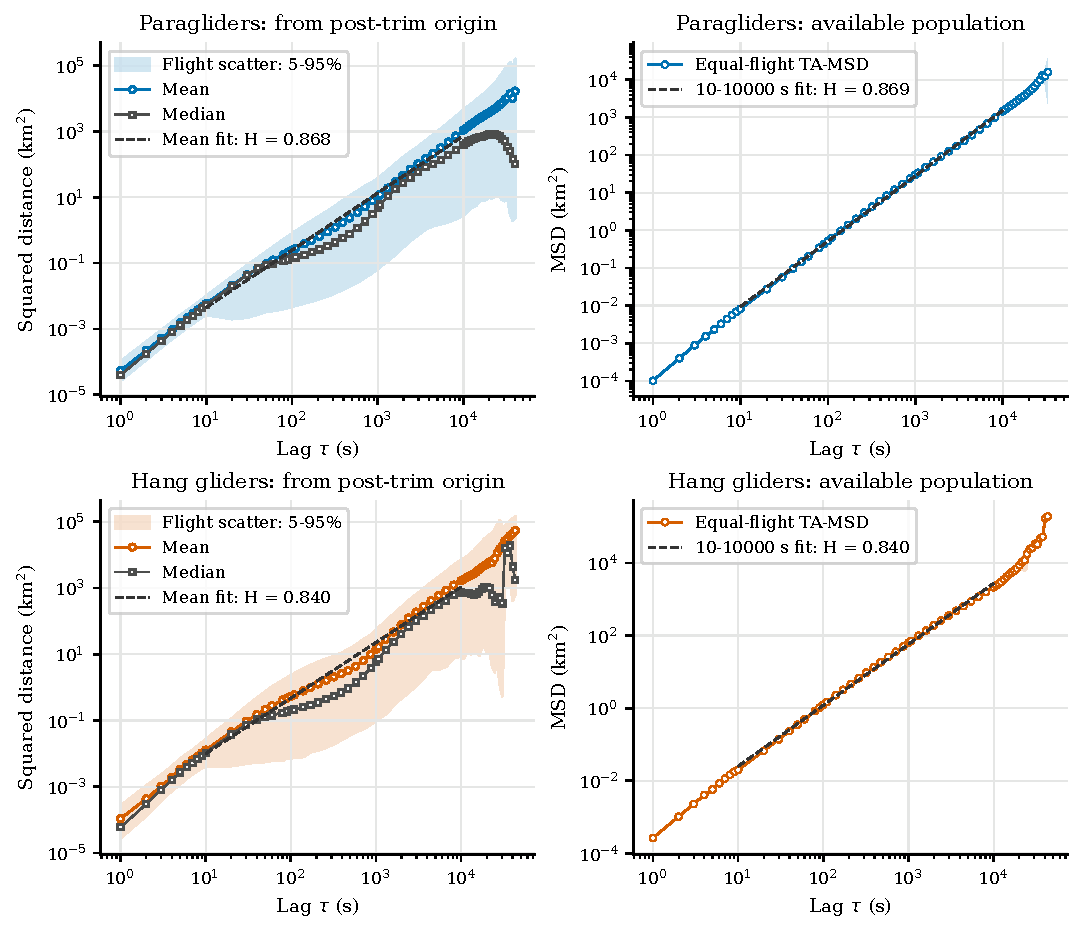
\includegraphics[width=\textwidth]{generated/ch3_transport_general.pdf}
 \caption{General horizontal transport. Left: squared distance from the post-trim
 origin, with equal-flight mean, median and the empirical 5--95\% flight range.
 Right: equal-flight TA-MSD over the population available at each lag, with
 pointwise 90\% cluster-bootstrap intervals and a log--log fit over 10--30000 s
 (evaluated lags: 10--28440 s). Native short-lag support differs from common-grid support.}
 \label{fig:fixed-general}
\end{figure}
The available-population fits give $H=0.869 [0.864, 0.874]$ for paragliders and $H=0.841 [0.816, 0.855]$ for hang gliders. These summarise growth with changing flight support. The hang-glider fit reaches a tail supported by only 7 groups; its interval uses 998 replicates with complete lag support.

\begin{table}[htbp]
 \centering\small
 \begin{tabular}{lrrr}
\toprule
Discipline & Lag (s) & TA-MSD flights & Origin-distance flights\\
\midrule
Paragliders & 10 & 155,085 & 152,771\\
Paragliders & 100 & 155,044 & 155,117\\
Paragliders & 1000 & 154,482 & 155,250\\
Paragliders & 10000 & 46,273 & 72,160\\
Paragliders & 32690 & 27 & 1,237\\
Hang gliders & 10 & 6,060 & 5,330\\
Hang gliders & 100 & 6,060 & 6,059\\
Hang gliders & 1000 & 6,044 & 6,070\\
Hang gliders & 10000 & 2,326 & 3,480\\
Hang gliders & 43200 & 1 & 3\\
\bottomrule
\end{tabular}

 \caption{Number of contributing flights in the general curves. The last row for
 each discipline is the largest evaluated lag with TA-MSD support. The origin-distance
 curve uses elapsed time; the TA-MSD requires a within-segment lag no larger than
 $0.8T_s$. Their support sets therefore differ. Early origin-distance support can increase
 when elapsed time exceeds an initial excluded interval or resolves a coarse cadence.}
 \label{tab:fixed-support}
\end{table}

\Needspace{20\baselineskip}
For a second-moment curve the local growth exponent is
\begin{equation}
 H_{\rm loc}(\tau)=\frac12\frac{d\log M_2(\tau)}{d\log\tau}.
 \label{eq:fixed-local-h}
\end{equation}
We estimate this derivative by a local log--log least-squares slope, divided by two,
within $\pm0.25$ decades of each lag and using at least three points.
In the general curves, a sparse interior window expands to the three nearest
log-lags: the estimate at 20 s uses the values at 10, 20 and 30 s.
For a single exponent over a specified interval, write $x_k=\log_{10}(\tau_k/1\,\mathrm{s})$.
The equal-weight least-squares slope of a dimensionless logarithmic ordinate $z_k$ is
\begin{equation}
 \mathcal B[z]=\frac{\sum_k(x_k-\bar x)z_k}{\sum_k(x_k-\bar x)^2},\qquad
 H=\frac12\mathcal B\!\left[\log_{10}\frac{M_2}{1\,\mathrm{m}^2}\right].
 \label{eq:fixed-fit}
\end{equation}
We fit the controlled analysis over 10--10000 s and refit every bootstrap curve to
propagate dependence between lags. The RMS logarithmic residual, in dex, measures
the departure from a single power law. Here $H$ denotes an effective growth exponent;
its identification with a process's self-similarity exponent is tested in
Section~\ref{sec:fixed-scaling}.

\begin{figure}[htbp]
 \centering
 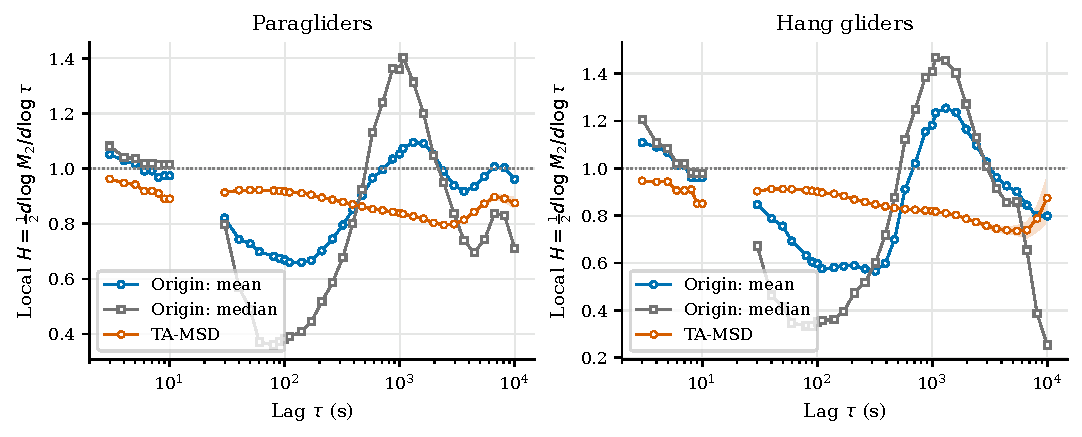
\includegraphics[width=\textwidth]{generated/ch3_transport_general_slopes.pdf}
 \caption{Local slopes of the general curves. The origin-distance mean and median
 have no confidence band here; the TA-MSD band is obtained by refitting bootstrap
 curves. The dotted reference is ballistic growth, $H=1$.}
 \label{fig:fixed-general-slopes}
\end{figure}
For paragliders, the origin-distance mean has an early local-slope minimum at the evaluated lag 110 s, with $H_{\rm loc}=0.66$ (search interval 20--2000 s).

For hang gliders, the origin-distance mean has an early local-slope minimum at the evaluated lag 320 s, with $H_{\rm loc}=0.57$ (search interval 20--2000 s).

Both curves are approximately ballistic at the earliest resolved lags and recover towards $H_{\rm loc}\simeq1$ around 600--700 s (Fig.~\ref{fig:fixed-general-slopes}).

The reduced growth after the initial ballistic regime is consistent with searching
for lift and climbing in a thermal, followed by renewed gliding. Under this
interpretation, the minimum marks a rough transition time towards completion of the
initial search-and-climb phase. It is distinct from the later recovery towards
$H_{\rm loc}=1$ and does not estimate a mean duration measured on individual flights.
The mean lies above the median, showing the influence of large displacements;
the pointwise percentiles do not track the same flights through time.

\FloatBarrier

\subsection{Fixed population and the effect of duration selection}
\label{sec:fixed-population}

As lag increases, short flights and segments leave the general average. A changing
mix of circuit types and launch sites can then alter its slope. For controlled
comparisons we select the segments once, using
\begin{equation}
 \tau_{\max}\leq0.8T_s,\qquad
 \mathcal C_{\tau_{\max}}=\{f:\exists s\in f,\ T_s\geq\tau_{\max}/0.8\},
 \label{eq:fixed-support}
\end{equation}
where $T_s$ is the segment's elapsed duration on the 10 s grid. This leaves at least
one fifth of that duration available for origins at the largest lag. The main cohort,
$\mathcal C_{10000}$, uses segments lasting at least 12500 s. If a flight has segments
of 14000 and 3000 s, only the first contributes, even at $\tau=10$ s.
Flights and selected segments therefore remain the same at every lag. The number of
increments still decreases with lag; dividing the flight's mass between them gives
\begin{equation}
 w_{fi}(\tau)=\frac{1}{Nn_f(\tau)},\qquad
 \sum_iw_{fi}(\tau)=\frac1N,\qquad N=|\mathcal C_{10000}|.
 \label{eq:fixed-weights}
\end{equation}

\begin{table}[htbp]
 \centering\small
 \begin{tabular}{llrrr}
\toprule
Discipline & $\tau_{\max}$ (s) & Flights & Segments & Groups\\
\midrule
Paragliders & 100 & 155,044 & 188,312 & 82,650\\
Paragliders & 1000 & 154,482 & 167,152 & 82,390\\
Paragliders & 10000 & 46,273 & 46,367 & 25,682\\
Hang gliders & 100 & 6,060 & 7,515 & 4,264\\
Hang gliders & 1000 & 6,044 & 6,610 & 4,253\\
Hang gliders & 10000 & 2,326 & 2,327 & 1,768\\
\bottomrule
\end{tabular}

 \caption{Nested duration cohorts and their site--day groups. Minimum segment
 durations are 125, 1250 and 12500 s, rounded upward when required by the 10 s grid.
 Existing cleaning and segment-admission conditions also apply. Flight and segment
 identities are retained in the numerical cohort manifests.}
 \label{tab:fixed-cohorts}
\end{table}

We assess duration selection with the nested cohorts $\mathcal C_{100}$ and
$\mathcal C_{1000}$. They contain the main cohort's segments, additional shorter
segments of its flights, and additional flights. We compare fitted $H$ over the same
lag interval, using paired bootstrap draws. The closed-route fraction changes from 56.6\% in $\mathcal C_{100}$ to 61.0\% in $\mathcal C_{10000}$ for paragliders. Thus duration selection measurably changes circuit composition.

The closed-route fraction changes from 64.0\% in $\mathcal C_{100}$ to 76.5\% in $\mathcal C_{10000}$ for hang gliders. Thus duration selection measurably changes circuit composition.


\begin{figure}[htbp]
 \centering
 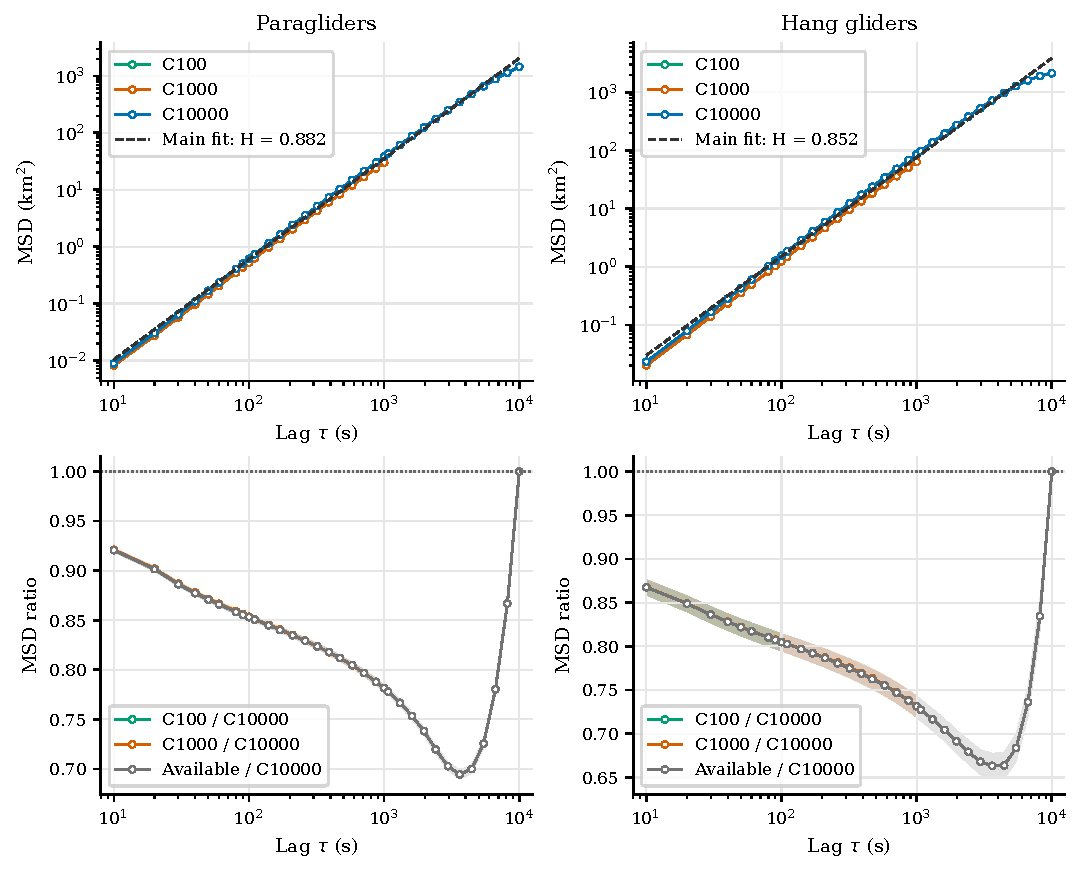
\includegraphics[width=\textwidth]{generated/ch3_transport_cohorts.pdf}
 \caption{Effect of duration selection. Top: MSD in the three nested cohorts;
 dashed lines fit the main cohort over 10--10000 s. Bottom: effective $H$ with 90\%
 intervals, fitted over 10--100 s for all three cohorts and 10--1000 s for the two
 longer cohorts. Fits within each comparison use identical lag values.}
 \label{fig:fixed-cohorts}
\end{figure}
\begin{table}[htbp]
 \centering\small
 \begin{tabular}{lllr}
\toprule
Discipline & Fit range (s) & Contrast & $\Delta H$ [5--95\%]\\
\midrule
Paragliders & 10--100 & $H_{\mathcal C_{100}}-H_{\mathcal C_{1000}}$ & -0.00006 [-0.00009, -0.00004]\\
Paragliders & 10--100 & $H_{\mathcal C_{100}}-H_{\mathcal C_{10000}}$ & -0.01687 [-0.01712, -0.01660]\\
Paragliders & 10--100 & $H_{\mathcal C_{1000}}-H_{\mathcal C_{10000}}$ & -0.01680 [-0.01705, -0.01654]\\
Paragliders & 10--1000 & $H_{\mathcal C_{1000}}-H_{\mathcal C_{10000}}$ & -0.01703 [-0.01733, -0.01674]\\
Hang gliders & 10--100 & $H_{\mathcal C_{100}}-H_{\mathcal C_{1000}}$ & -0.00002 [-0.00013, 0.00011]\\
Hang gliders & 10--100 & $H_{\mathcal C_{100}}-H_{\mathcal C_{10000}}$ & -0.01646 [-0.01748, -0.01552]\\
Hang gliders & 10--100 & $H_{\mathcal C_{1000}}-H_{\mathcal C_{10000}}$ & -0.01644 [-0.01746, -0.01550]\\
Hang gliders & 10--1000 & $H_{\mathcal C_{1000}}-H_{\mathcal C_{10000}}$ & -0.01771 [-0.01879, -0.01668]\\
\bottomrule
\end{tabular}

 \caption{Paired differences of the cohort exponents in Fig.~\ref{fig:fixed-cohorts}.
 Each comparison uses identical lags and bootstrap draws. A 90\% interval excluding
 zero resolves a difference under the adopted resampling; inclusion of zero alone
 would not establish absence of selection bias.}
 \label{tab:fixed-cohort-fits}
\end{table}
For paragliders, the dedicated-to-main MSD ratio is 0.853 [0.851, 0.855] at 100 s and 0.781 [0.778, 0.785] at 1000 s. The long-flight requirement therefore selects larger mean displacements at shared lags, with differences exceeding the paired bootstrap variability.

For hang gliders, the dedicated-to-main MSD ratio is 0.805 [0.795, 0.814] at 100 s and 0.731 [0.719, 0.743] at 1000 s. The long-flight requirement therefore selects larger mean displacements at shared lags, with differences exceeding the paired bootstrap variability.

The resulting estimates remain conditional on long uninterrupted flight segments;
the shorter cohorts describe a broader flight population.

\FloatBarrier

\section{Transport by circuit type and initial altitude}
\label{sec:fixed-circuit}

The catalogue's declared circuit class separates open distance flights from closed
routes such as triangles and out-and-return flights. We cross this distinction with
initial cleaned GNSS altitude: Plains ($z_0<300$ m), Hills ($300\leq z_0<800$ m),
Low mountains ($800\leq z_0<1500$ m), and High mountains ($z_0\geq1500$ m).
These are launch-altitude classes; they do not classify the terrain crossed later.
This comparison uses paragliders and the same $\mathcal C_{10000}$ support rule in
all eight cells. Counts and fitted exponents are given in Table~\ref{tab:fixed-task}.
The eligible common-grid population contains 67,003 open flights (43.2\%), 87,807 closed flights (56.6\%), and 275 without a recognised circuit class.

The main cohort contains 17,961 open flights (38.8\%), 28,234 closed flights (61.0\%), and 78 without a recognised circuit class.


\begin{figure}[htbp]
 \centering
 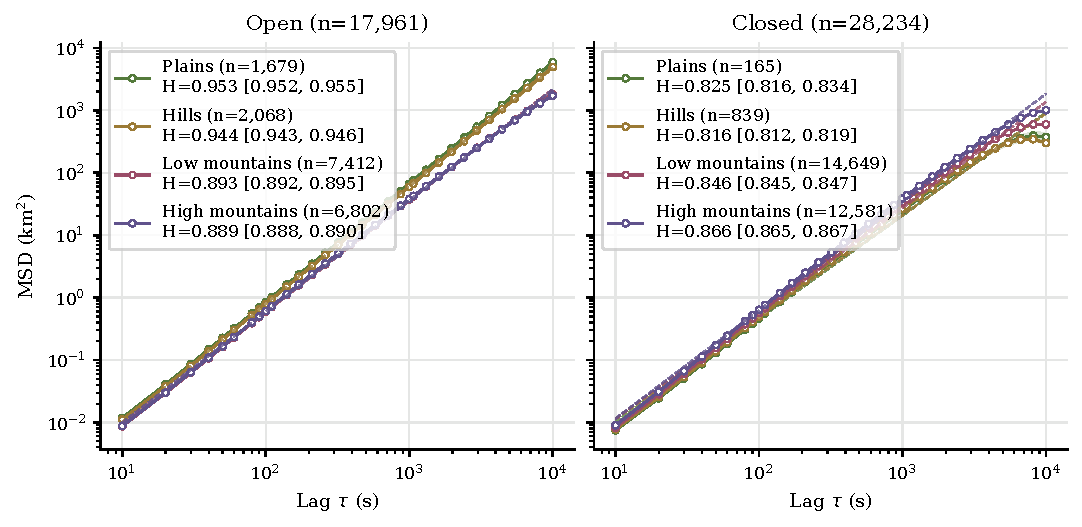
\includegraphics[width=\textwidth]{generated/ch3_transport_task_altitude.pdf}
 \caption{Paraglider transport by declared circuit and initial altitude, with fixed
 flights and segments throughout 10--10000 s. Markers give MSD estimates, shaded
 bands their pointwise 90\% intervals, and dashed lines the global log--log fits.
 The identical axes permit comparison of displacement amplitude and growth rate.}
 \label{fig:fixed-task}
\end{figure}
\begin{table}[htbp]
 \centering\footnotesize\setlength{\tabcolsep}{3.5pt}
 \begin{tabular}{llrrrr}
\toprule
Circuit & Initial altitude & $N$ & $G$ & $H$ [5--95\%] & $M_2(10^4)$ (km$^2$)\\
\midrule
Open & Plains & 1,679 & 1,140 & 0.953 [0.952, 0.955] & 5900\\
Open & Hills & 2,068 & 1,634 & 0.944 [0.943, 0.946] & 4920\\
Open & Low mountains & 7,412 & 5,255 & 0.893 [0.892, 0.895] & 1814\\
Open & High mountains & 6,802 & 4,794 & 0.889 [0.888, 0.890] & 1710\\
Closed & Plains & 165 & 157 & 0.825 [0.816, 0.834] & 372\\
Closed & Hills & 839 & 756 & 0.816 [0.812, 0.819] & 299\\
Closed & Low mountains & 14,649 & 7,954 & 0.846 [0.845, 0.847] & 596\\
Closed & High mountains & 12,581 & 7,406 & 0.866 [0.865, 0.867] & 1001\\
\bottomrule
\end{tabular}

 \caption{Main-cohort flights $N$, site--day groups $G$, global effective exponents
 and displacement amplitude at 10000 s. Intervals come from the coupled cluster
 bootstrap. Even the smallest cell retains 165 flights from 157 groups.}
 \label{tab:fixed-task}
\end{table}

For open routes, Plains and Hills have larger $H$ than either mountain class. Thus
the distinction involves the rate of growth as well as the displacement reached at
10000 s. Closed routes have smaller $H$ than open routes in every altitude class.
The paired contrasts $H_{\rm open}-H_{\rm closed}$ range from 0.023 to 0.129; all four 90\% intervals exclude zero.

The closed-route exponents also differ between altitude classes: the present intervals
do not support a common value across them.

A return objective can suppress net
horizontal advance on scales approaching a circuit's duration, although the declared
class does not guarantee exact closure of the trimmed trajectory. Faster displacement growth
in low-altitude open flights is consistent with fewer topographic constraints on
horizontal progression. This observational comparison does not isolate orography
from weather, route selection, pilots or equipment.

Within the fixed cohort the group fractions $p_g=N_g/N$ are constant. For an
exhaustive partition, including unclassified flights,
\begin{equation}
 M_2(\tau)=\sum_g p_g M_{2,g}(\tau),\qquad
 H_{\rm loc}(\tau)=\sum_g
 \frac{p_gM_{2,g}(\tau)}{M_2(\tau)}H_{{\rm loc},g}(\tau).
 \label{eq:fixed-mixture}
\end{equation}
The derivative slope weights each group by its contribution to the second moment.
Equation~\eqref{eq:fixed-mixture} describes the main-cohort MSD; the plotted local
regressions approximate its derivatives. Both circuit classes contribute substantially
to this aggregate, with distinct growth rates.

Wind can contribute to both amplitude and apparent scaling. For an additive constant
velocity $\boldsymbol u$, write $\Delta\boldsymbol x=\Delta\boldsymbol y+\boldsymbol u\tau$:
\begin{equation}
 \langle|\Delta\boldsymbol x|^2\rangle
 =\langle|\Delta\boldsymbol y|^2\rangle
 +2\tau\boldsymbol u\cdot\langle\Delta\boldsymbol y\rangle+|\boldsymbol u|^2\tau^2.
 \label{eq:fixed-wind}
\end{equation}
Even a uniform constant drift can change the slope of this uncentred MSD through its
ballistic term. A common deterministic shift cancels from the centred covariance;
drifts differing between flights need not cancel from the mixture. A variable wind
field can additionally modify velocity correlations. Wind is not separated quantitatively
in this comparison.
\FloatBarrier

\section{Anisotropy and principal directions}
\label{sec:fixed-anisotropy}
\emph{Reserved for the analysis of anisotropy and principal directions. The existing
PCA results remain in the experiments volume; they are not updated in this chapter.}

\section{Scaling of displacement distributions}
\label{sec:fixed-scaling}

The MSD measures one moment of the displacement law. To test whether the whole law
rescales with one exponent, we use quantiles, a spectrum of moments and excess kurtosis.
All use the main cohort's flights, segments and weights in Eq.~\eqref{eq:fixed-weights}.

\subsection{Self-similarity and its observable consequences}
\label{sec:fixed-selfsimilar-definition}

A process $\boldsymbol X(t)$, with $\boldsymbol X(0)=0$, is $H$-self-similar if,
for some $H>0$,
\begin{equation}
 \bigl(\boldsymbol X(at_1),\ldots,\boldsymbol X(at_m)\bigr)
 \overset d= a^H\bigl(\boldsymbol X(t_1),\ldots,\boldsymbol X(t_m)\bigr)
 \quad(a>0).
 \label{eq:fixed-selfsimilar}
\end{equation}
This identity must hold for every $m\geq1$ and $t_1,\ldots,t_m\geq0$.
Equality in distribution concerns positions at any collection of times, including
their dependence~\cite{embrechts_maejima_selfsimilar}. Gaussianity and independence
of increments are not required.

To infer a lag-only scaling law, we additionally assume stationary increments:
their joint laws must be unchanged by shifting the origin.
Self-similarity alone does not impose this condition. With stationary increments,
each amplitude $Y\in\{|\Delta E|,|\Delta N|,R\}$ obeys
\begin{equation}
 Y(\tau)\overset d=(\tau/\tau_0)^H Y(\tau_0),\qquad
 \begin{aligned}
 Q_{Y,p}(\tau)&=(\tau/\tau_0)^H Q_{Y,p}(\tau_0),\\
 M_{q,Y}(\tau)&=(\tau/\tau_0)^{qH}M_{q,Y}(\tau_0).
 \end{aligned}
 \label{eq:fixed-scale-family}
\end{equation}
Here $Q_{Y,p}$ is a population quantile and $M_{q,Y}$ a finite moment of order $q$;
below, the same symbols denote their equal-flight estimates.
Thus every quantile has the same exponent, quantile ratios are constant, and the
moment spectrum is $\zeta_Y(q)=qH$. Signed-component excess kurtosis is also constant
when the fourth moment exists and variance is nonzero; it need not vanish. These are
necessary consequences for the lag distributions. A finite selection of such
statistics cannot establish the joint-law identity in Eq.~\eqref{eq:fixed-selfsimilar}.

\subsection{A common empirical distribution}

With the weights in Eq.~\eqref{eq:fixed-weights}, the common empirical distribution is
\begin{equation}
 \widehat F_{Y,\tau}(y)=\frac1N\sum_{f=1}^N\frac1{n_f(\tau)}
 \sum_{i=1}^{n_f(\tau)}\mathbf1\{Y_{fi}(\tau)\leq y\},\qquad
 Q_{Y,p}(\tau)=\inf\{y:\widehat F_{Y,\tau}(y)\geq p\}.
 \label{eq:fixed-cdf}
\end{equation}
We average the within-flight fractions below $y$, then invert the resulting CDF.
The quantile is the first observed amplitude at which the cumulative weight reaches
$p$, without interpolation between ranks. This order of operations defines the
quantile of the equal-flight mixture.

Absolute components measure amplitudes along east and north. For example,
$\Pr(|\Delta E|\leq a)=\Pr(-a\leq\Delta E\leq a)$, so small absolute quantiles
measure proximity to zero displacement. The radius $R=(\Delta E^2+\Delta N^2)^{1/2}$
is invariant under rotation and measures horizontal displacement without assuming
isotropy.

\subsection{Quantiles, growth exponents and relative spread}
\label{sec:fixed-quantiles}

We evaluate $p=0.25,0.50,0.75,0.90$ and fit each quantile over the same 33 lags.
Using the slope operator in Eq.~\eqref{eq:fixed-fit},
\begin{equation}
 H_{Y,p}=\mathcal B\!\left[\log_{10}\frac{Q_{Y,p}}{1\,\mathrm m}\right],\qquad
 \mathcal B\!\left[\log_{10}\frac{Q_{Y,0.25}}{Q_{Y,0.90}}\right]
 =H_{Y,0.25}-H_{Y,0.90}.
 \label{eq:fixed-ratio}
\end{equation}
No factor of two enters a length exponent. The ratio compares small and large
amplitudes at each lag, while the fitted exponents summarise their growth across
10--10000 s. The equality follows from linearity of least squares on identical lags;
ratio drift and the exponent difference are therefore linked diagnostics.

\begin{figure}[H]
 \centering
 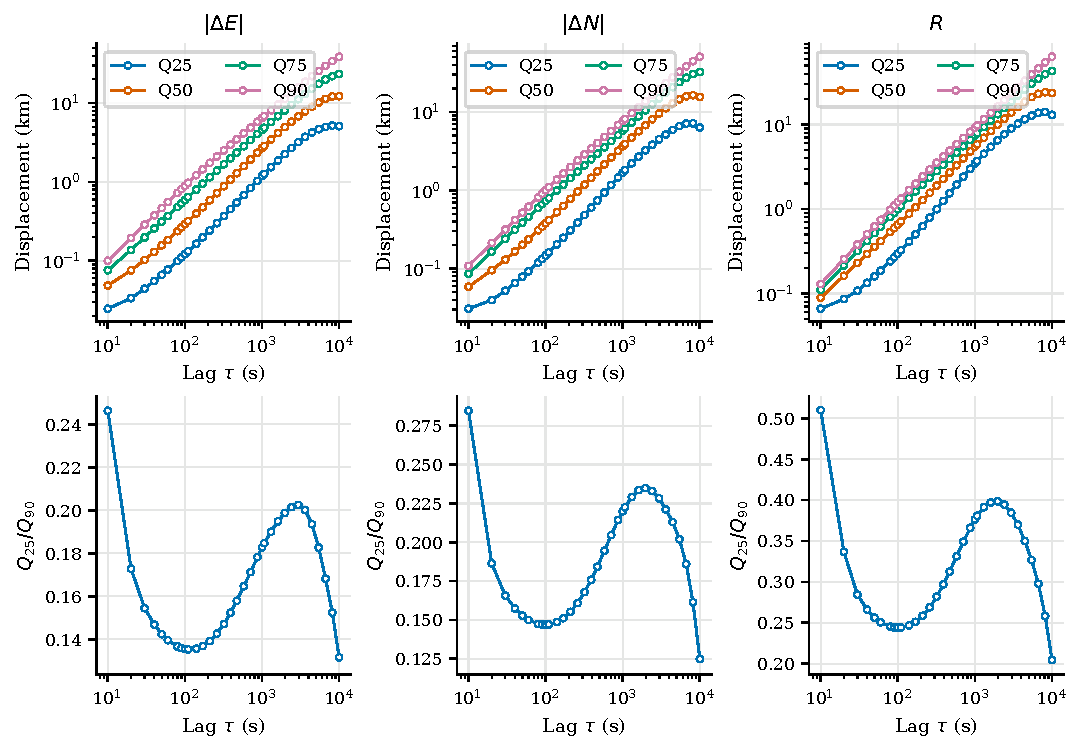
\includegraphics[width=\textwidth]{generated/ch3_transport_quantiles_para.pdf}
 \caption{Paraglider equal-flight displacement quantiles and their relative spread,
 on the fixed main cohort. Every panel uses the empirical measure in
 Eq.~\eqref{eq:fixed-cdf}. Shading gives pointwise 90\% cluster-bootstrap intervals.}
 \label{fig:fixed-quantiles-para}
\end{figure}
\begin{figure}[htbp]
 \centering
 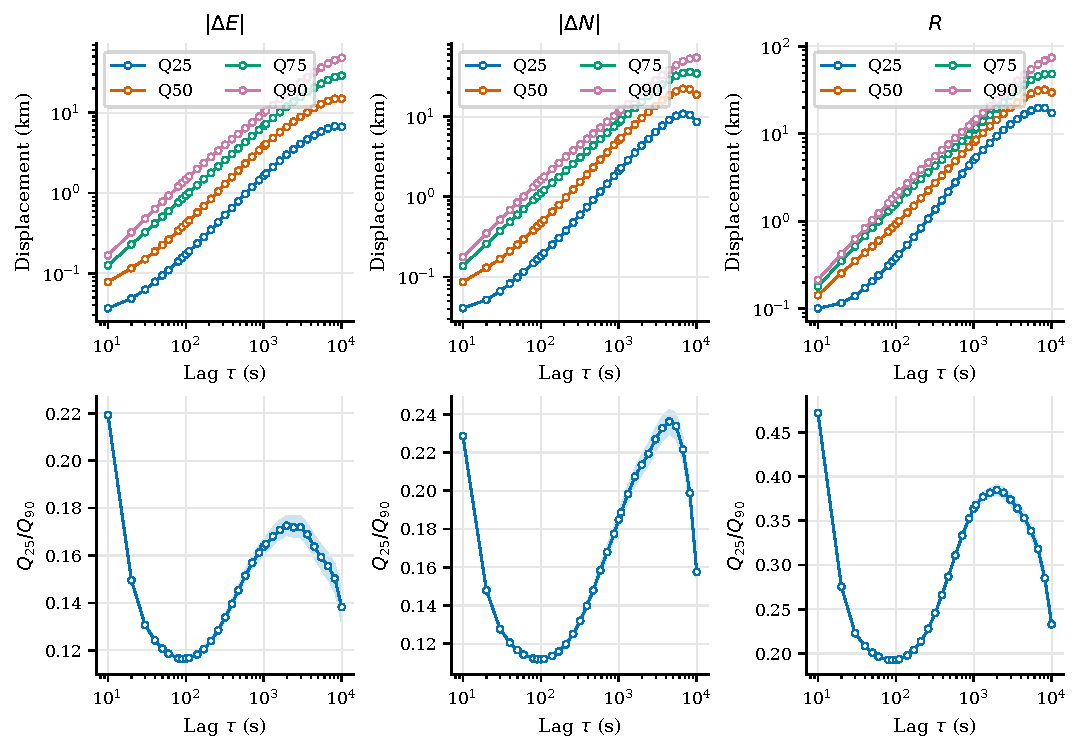
\includegraphics[width=\textwidth]{generated/ch3_transport_quantiles_hang.pdf}
 \caption{The same amplitude quantiles and ratio for hang gliders, with an independent
 main cohort and the same sampling convention.}
 \label{fig:fixed-quantiles-hang}
\end{figure}
\begin{figure}[htbp]
 \centering
 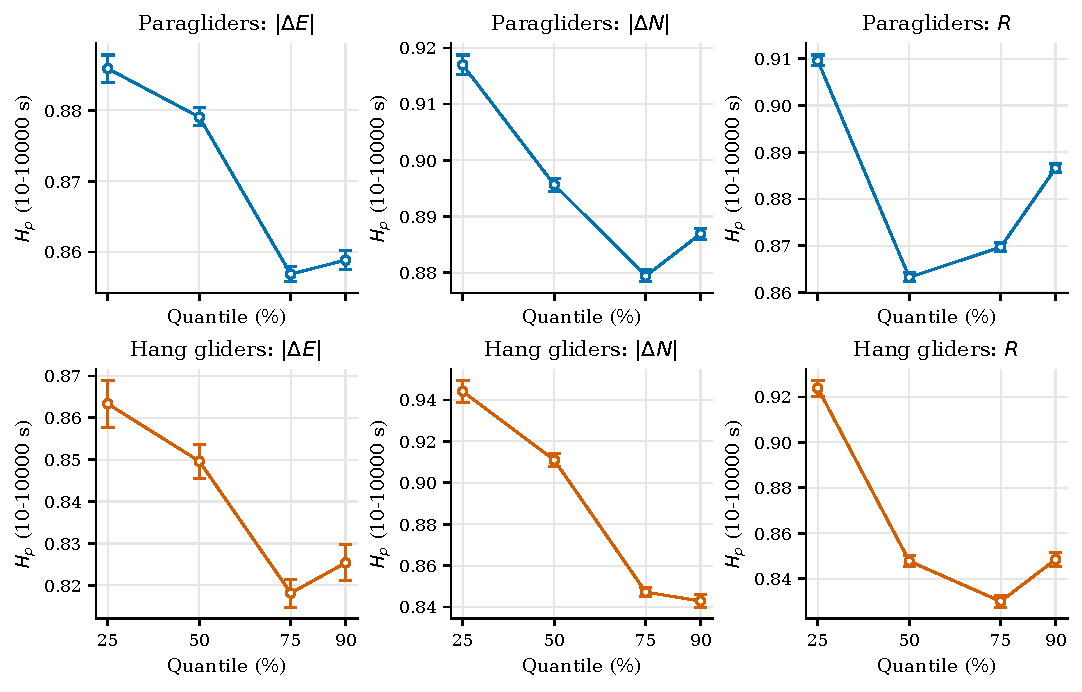
\includegraphics[width=\textwidth]{generated/ch3_transport_quantile_exponents.pdf}
 \caption{Global quantile exponents from 10--10000 s fits. Error bars are the 5th--95th
 percentiles of the refitted bootstrap slopes. A common scale exponent would give
 a horizontal sequence within each panel.}
 \label{fig:fixed-quantile-h}
\end{figure}
For paragliders, the radial ratio is 0.510 at 10 s, has an early minimum of 0.244 at 100 s, and takes the value 0.398 at 1970 s before ending at 0.205 at 10000 s. The global radial contrast $H_{25}-H_{90}$ is 0.023 [0.022, 0.024]. Quantile-fit RMS residuals span 0.023--0.084 dex.

For hang gliders, the radial ratio is 0.472 at 10 s, has an early minimum of 0.192 at 90 s, and takes the value 0.385 at 1970 s before ending at 0.233 at 10000 s. The global radial contrast $H_{25}-H_{90}$ is 0.075 [0.071, 0.079]. Quantile-fit RMS residuals span 0.037--0.101 dex.

The nonmonotonic ratios show changes of distributional shape across scales. A global positive ratio slope summarises all fitted lags and need not imply a net increase between the two endpoints. The effective quantile exponents must therefore be read together with the curves.

\FloatBarrier

\subsection{Moment spectrum and finite-range scaling}
\label{sec:fixed-moments}

For each amplitude and order we calculate
\begin{equation}
 M_{q,Y}(\tau)=\frac1N\sum_f\frac1{n_f(\tau)}\sum_iY_{fi}(\tau)^q,
 \qquad \zeta_Y(q)=\mathcal B\!\left[\log_{10}\frac{M_{q,Y}}{(1\,\mathrm m)^q}\right].
 \label{eq:fixed-moments}
\end{equation}
We use $q\in\{0.25,0.5,0.75,1,1.5,2,2.5,3,3.5,4\}$. Each point of the spectrum is
obtained by first computing a moment at all lags, then fitting its log--log slope.
The reference $\zeta=qH$ is fitted through the origin with equal weight for the ten
orders. Higher orders emphasise large displacements. The radial spectrum contains
the MSD, with the identity
\begin{equation}
 M_{2,R}=M_{2,|\Delta E|}+M_{2,|\Delta N|}=M_2
 \label{eq:fixed-second-identity}
\end{equation}
verified at every lag and in every bootstrap replicate.

\begin{table}[htbp]
 \centering\small
 \begin{tabular}{llrr}
\toprule
Discipline & Fit range (s) & $H$ [5--95\%] & RMS (dex)\\
\midrule
Paragliders & 10--10000 & 0.882 [0.881, 0.883] & 0.046\\
Paragliders & 10--100 & 0.925 [0.924, 0.925] & 0.007\\
Paragliders & 100--1000 & 0.898 [0.897, 0.898] & 0.006\\
Paragliders & 1000--10000 & 0.804 [0.802, 0.807] & 0.026\\
Hang gliders & 10--10000 & 0.852 [0.849, 0.855] & 0.072\\
Hang gliders & 10--100 & 0.915 [0.914, 0.916] & 0.006\\
Hang gliders & 100--1000 & 0.873 [0.871, 0.874] & 0.007\\
Hang gliders & 1000--10000 & 0.728 [0.720, 0.737] & 0.051\\
\bottomrule
\end{tabular}

 \caption{Main-cohort MSD exponents: a single global fit and three common decade
 intervals. RMS residuals are measured in $\log_{10}M_2$. Each fit retains the same
 flight and segment population.}
 \label{tab:fixed-fits}
\end{table}
\begin{figure}[htbp]
 \centering
 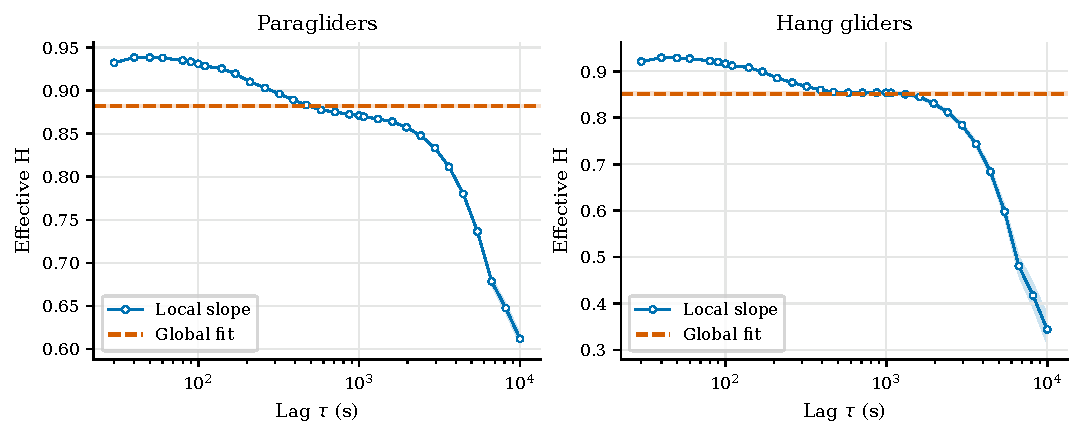
\includegraphics[width=\textwidth]{generated/ch3_transport_fixed_slopes.pdf}
 \caption{Local and global effective MSD exponents on the fixed main cohort.
 Bands are pointwise 90\% bootstrap intervals. The global fit compresses the full
 curve into one number; the local slopes expose its scale dependence.}
 \label{fig:fixed-local}
\end{figure}
\begin{figure}[htbp]
 \centering
 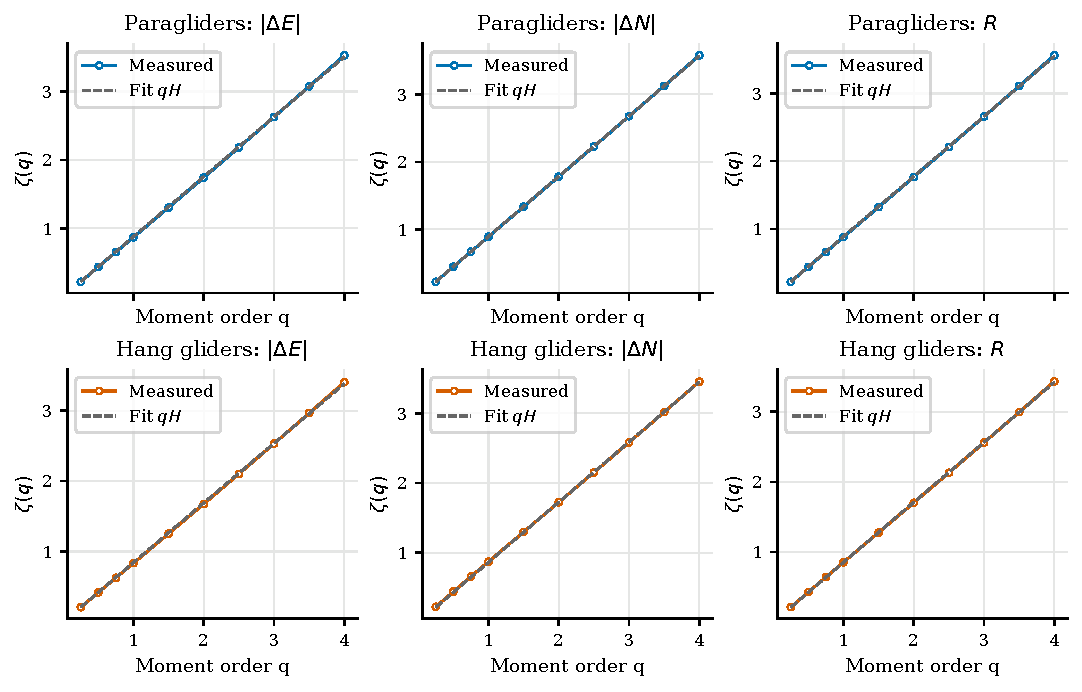
\includegraphics[width=\textwidth]{generated/ch3_transport_spectrum.pdf}
 \caption{Moment spectra for the three displacement amplitudes. Each point is the
 slope of a 10--10000 s log--log moment fit; shading gives its pointwise 90\% interval.
 Dashed lines are constrained linear fits $\zeta=qH$.}
 \label{fig:fixed-spectrum}
\end{figure}
\begin{table}[htbp]
 \centering\small\setlength{\tabcolsep}{4pt}
 \begin{tabular}{llrr}
\toprule
Discipline & Amplitude & $H_{25}-H_{90}$ & $\zeta(4)/4-\zeta(0.25)/0.25$\\
\midrule
Paragliders & $|\Delta E|$ & 0.027 [0.025, 0.029] & 0.0113 [0.0097, 0.0128]\\
Paragliders & $|\Delta N|$ & 0.030 [0.028, 0.032] & -0.0004 [-0.0016, 0.0009]\\
Paragliders & $R$ & 0.023 [0.022, 0.024] & 0.0095 [0.0086, 0.0105]\\
Hang gliders & $|\Delta E|$ & 0.038 [0.032, 0.044] & 0.0095 [0.0040, 0.0150]\\
Hang gliders & $|\Delta N|$ & 0.101 [0.096, 0.106] & -0.0269 [-0.0305, -0.0232]\\
Hang gliders & $R$ & 0.075 [0.071, 0.079] & -0.0085 [-0.0112, -0.0057]\\
\bottomrule
\end{tabular}

 \caption{Paired global-slope contrasts, with 5--95\% bootstrap intervals. A common
 scale exponent predicts zero for both the quantile and moment contrasts.}
 \label{tab:fixed-scaling}
\end{table}
The single global MSD exponent is $H=0.882 [0.881, 0.883]$ for paragliders. The radial contrast $\zeta(4)/4-\zeta(0.25)/0.25$ is 0.0095 [0.0086, 0.0105]; across all three amplitudes and orders, moment-fit RMS residuals range from 0.010 to 0.079 dex.

The single global MSD exponent is $H=0.852 [0.849, 0.855]$ for hang gliders. The radial contrast $\zeta(4)/4-\zeta(0.25)/0.25$ is -0.0085 [-0.0112, -0.0057]; across all three amplitudes and orders, moment-fit RMS residuals range from 0.011 to 0.126 dex.

The decade fits and local slopes expose crossovers within the full interval. Accordingly, a small departure of the fitted spectrum from $qH$ is evidence against a common effective exponent on these scales, rather than a measurement of an asymptotic multifractal law.

\FloatBarrier

\subsection{Excess kurtosis of the signed components}
\label{sec:fixed-kurtosis}

Departures from Gaussian shape are assessed on the signed components: taking an
absolute value or a radius changes even a Gaussian law. With the equal-flight mean
$\langle A\rangle_\tau=\sum_{f,i}w_{fi}(\tau)A_{fi}$, define
\begin{equation}
 \mu_j(\tau)=\langle\Delta x_j\rangle_\tau,\qquad
 K_j(\tau)=\frac{\langle(\Delta x_j-\mu_j)^4\rangle_\tau}
 {\langle(\Delta x_j-\mu_j)^2\rangle_\tau^2}-3,\qquad j\in\{E,N\}.
 \label{eq:fixed-kurtosis}
\end{equation}
Centring uses the mean of the full mixture at each lag. A Gaussian marginal has
$K_j=0$~\cite{nist_kurtosis}; nonzero excess measures a departure in its standardised
fourth moment. Zero excess alone does not establish Gaussianity. For self-similarity,
the relevant prediction is constancy with lag, regardless of the value.

\begin{figure}[htbp]
 \centering
 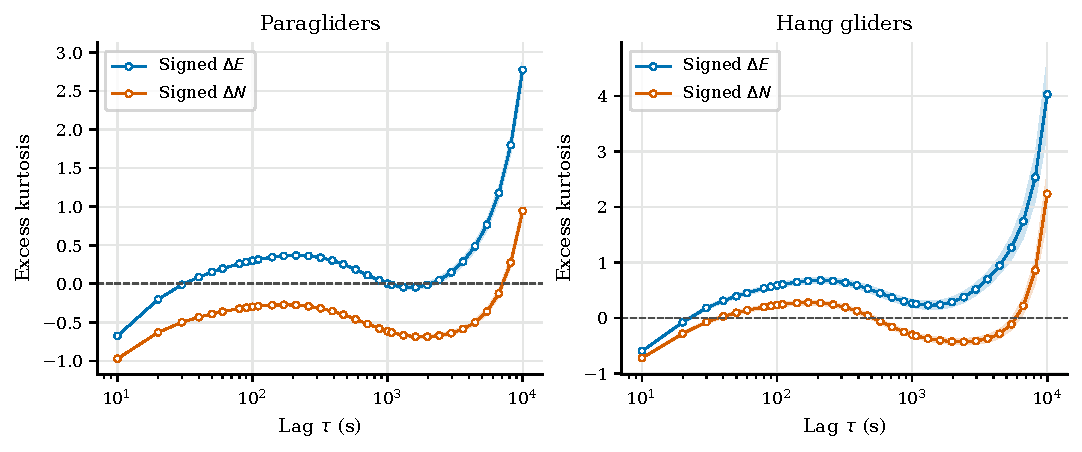
\includegraphics[width=\textwidth]{generated/ch3_transport_kurtosis.pdf}
 \caption{Signed-component Fisher excess kurtosis at the same lags, with the same
 flights, segments and weights as the quantiles and moments. The dashed line is the
 Gaussian marginal reference. Bands use the coupled cluster bootstrap.}
 \label{fig:fixed-kurtosis}
\end{figure}
For paragliders, $(K_E,K_N)$ changes from $(-0.68,-0.97)$ at 10 s to $(2.77,0.94)$ at 10000 s. The short-lag negative excess and long-lag positive excess show a change in standardised fourth-moment shape.

For hang gliders, $(K_E,K_N)$ changes from $(-0.60,-0.72)$ at 10 s to $(4.03,2.24)$ at 10000 s. The short-lag negative excess and long-lag positive excess show a change in standardised fourth-moment shape.

Different flight means and variances can themselves produce nonzero excess in the
mixture. The measured kurtosis therefore characterises the pooled displacement law.

\subsection{Assessment of self-similarity}

The quantile curves and the nearly straight moment spectra can be reconciled through
\begin{equation}
 M_{q,Y}(\tau)=\int_0^1 Q_{Y,p}(\tau)^q\,dp.
 \label{eq:fixed-moment-quantile}
\end{equation}
Each moment averages over probability levels; the order $q$ controls the emphasis
on larger amplitudes. Fitting its slope
across three decades further averages over crossovers. Changes in different parts
of the distribution can consequently leave the fitted spectrum nearly linear.
Moreover, Table~\ref{tab:fixed-scaling} resolves small departures from $\zeta=qH$;
the spectrum is not exactly linear under the adopted bootstrap.

For these data, the lag-dependent quantile ratios provide the more direct evidence
against a fixed distributional shape. Their large, nonmonotonic changes are visible
without fitting a power law, and their estimation does not require finite high-order
moments. Unequal fitted quantile exponents support this reading, but the curved
quantile trajectories limit their interpretation as constant exponents. The change
in kurtosis supplies complementary evidence. Visual linearity of ten fitted moment
slopes is therefore insufficient to outweigh the observed shape changes.

The finite-range evidence does not support one common displacement scale exponent over 10--10000 s: quantile ratios vary, fitted quantile slopes differ, and standardised fourth moments change with lag. The global MSD exponent remains a useful summary of net growth. Approximate linearity of a moment spectrum alone does not establish monofractal scaling across an interval containing these crossovers.

Approximate scaling over narrower intervals remains possible. Fixed flights and
segments remove changing membership, but the available origins still change with lag
and may sample flight phases differently. The present analysis does not separate
this effect from within-flight dynamics or determine multi-time laws. It therefore
does not exclude every nonstationary self-similar process, nor establish an asymptotic
multifractal law.

\FloatBarrier
